\documentclass{article}
\usepackage{tikz}
\usepackage{geometry}
\geometry{a4paper, margin=0.5in}
\usetikzlibrary{shapes.geometric, arrows, positioning, shapes.misc}
\usepackage[normalem]{ulem}
\tikzset{
  multivalued attribute/.style={
    draw,
    ellipse,
    minimum width=3cm,
    minimum height=1.5cm,
    double,
    double distance=1pt
  }
}
\tikzset{
  weak relationship/.style={
    draw,
    diamond,
    double,
    double distance=1pt,
    minimum width=3cm,
    minimum height=1.5cm
  }
}
\tikzset{
  derived attribute/.style={ellipse, draw, dashed, minimum width=2cm, minimum height=1cm, align=center}
}

\begin{document}

% ============================================================================
% 6.1 Car Insurance Company ER Diagram
% ============================================================================
\section*{6.1 Car Insurance Company}
\begin{tikzpicture}[
    node distance=1.5cm,
    entity/.style={rectangle, draw, minimum width=2cm, minimum height=0.8cm, text centered},
    relationship/.style={diamond, draw, minimum width=2cm, minimum height=0.8cm, text centered},
    attribute/.style={ellipse, draw, minimum width=1.5cm, minimum height=0.6cm, text centered, font=\small},
    key/.style={ellipse, draw, minimum width=1.5cm, minimum height=0.6cm, text centered, font=\small, text decoration=underline}
]

% Entities
\node[entity] (customer) {Customer};
\node[entity, right=4cm of customer] (car) {Car};
\node[entity, right=4cm of car] (policy) {Insurance Policy};
\node[entity, below=2cm of policy] (payment) {premium payment};
\node[entity, below=2cm of car] (accident) {accident};

% Relationships
\node[relationship, right=2cm of customer] (owns) {owns};
\node[relationship, right=2cm of car] (covers) {covers};
\node[relationship, below=1cm of policy] (pays) {pays};
\node[relationship, below=1cm of car] (participated) {participated};

% Customer attributes
\node[key, above left=1cm of customer] (cust_id) {customer\_id};
\node[attribute, above=1cm of customer] (name) {name};
\node[attribute, above right=1cm of customer] (address) {address};

% Car attributes
\node[attribute, above left=1cm of car] (license) {license\_no};
\node[attribute, above right=1cm of car] (model) {model};

% Policy attributes  
\node[key, above=1cm of policy] (policy_id) {policy\_id};

% Payment attributes
\node[key, below left=1cm of payment] (payment_id) {payment\_id};
\node[attribute, below=1cm of payment] (due_date) {due\_date};
\node[attribute, below right=1cm of payment] (amount) {amount};

% Accident attributes
\node[key, below left=1cm of accident] (report_id) {report\_id};
\node[attribute, below=1cm of accident] (date) {date};
\node[attribute, below right=1cm of accident] (place) {place};

% Connections
\draw (customer) -- (owns);
\draw (owns) -- (car);
\draw (car) -- (covers);
\draw (covers) -- (policy);
\draw (policy) -- (pays);
\draw (pays) -- (payment);
\draw (car) -- (participated);
\draw (participated) -- (accident);

% Attribute connections
\draw (customer) -- (cust_id);
\draw (customer) -- (name);
\draw (customer) -- (address);
\draw (car) -- (license);
\draw (car) -- (model);
\draw (policy) -- (policy_id);
\draw (payment) -- (payment_id);
\draw (payment) -- (due_date);
\draw (payment) -- (amount);
\draw (accident) -- (report_id);
\draw (accident) -- (date);
\draw (accident) -- (place);

\end{tikzpicture}

\newpage

% ============================================================================
% 6.2 University Schema - Ternary Relationship
% ============================================================================
\section*{6.2 University Schema - Ternary Relationship}
\begin{tikzpicture}[
    node distance=2cm,
    entity/.style={rectangle, draw, minimum width=2cm, minimum height=0.8cm, text centered},
    relationship/.style={diamond, draw, minimum width=2cm, minimum height=0.8cm, text centered},
    attribute/.style={ellipse, draw, minimum width=1.5cm, minimum height=0.6cm, text centered, font=\small},
    key/.style={ellipse, draw, minimum width=1.5cm, minimum height=0.6cm, text centered, font=\small, text decoration=underline}
]

% Entities
\node[entity] (student) {student};
\node[entity, right=6cm of student] (section) {section};
\node[entity, above=3cm of section] (course) {course};


% Relationships
\node[relationship, right=2cm of student] (marks) {exam\_marks};
\node[weak relationship, above right=1.5cm of section] (sec_course) {sec\_course};

% Student attributes
\node[key, above left=1cm of student] (student_id) {\underline{student\_id}};
\node[attribute, above=1cm of student] (s_name) {name};
\node[attribute, left=1cm of student] (tot_cred) {tot\_cred};
\node[attribute, below left=1cm of student] (dept_name) {dept\_name};

% Section attributes
\node[attribute, right=1cm of section] (sec_id) {\dashuline{sec\_id}};
\node[attribute, below right=1cm of section] (semester) {\dashuline{semester}};
\node[attribute, below=1cm of section] (year) {\dashuline{year}};

% Course attributes
\node[key, above=1cm of course] (course_id) {\underline{course\_id}};
\node[attribute, above left=1cm of course] (title) {title};
\node[attribute, above right=1cm of course] (credits) {credits};

% Exam attributes
\node[key, below left=1cm of marks] (exam_id) {exam\_id};
\node[attribute, below=1cm of marks] (e_name) {name};


% Relationship attribute
\node[attribute, below right=1cm of marks] (exam_marks) {marks};

% Connections
\draw (student) -- (marks);
\draw (section) -- (marks);
\draw (section) -- (sec_course);
\draw (course) -- (sec_course);
\draw[dashed] (marks) -- (exam_marks);

% Attribute connections
\draw (student) -- (student_id);
\draw (student) -- (s_name);
\draw (student) -- (tot_cred);
\draw (student) -- (dept_name);
\draw (section) -- (sec_id);
\draw (section) -- (semester);
\draw (section) -- (year);
\draw (course) -- (course_id);
\draw (course) -- (title);
\draw (course) -- (credits);
\draw[dashed] (marks) -- (exam_id);
\draw[dashed] (marks) -- (e_name);


\end{tikzpicture}

\newpage

% ============================================================================
% 6.3 University Schema - Binary Relationship Alternative
% ============================================================================
\section*{6.3 University Schema - Binary Relationship Alternative}
\begin{tikzpicture}[
    node distance=2cm,
    entity/.style={rectangle, draw, minimum width=2cm, minimum height=0.8cm, text centered},
    relationship/.style={diamond, draw, minimum width=2cm, minimum height=0.8cm, text centered},
    attribute/.style={ellipse, draw, minimum width=1.5cm, minimum height=0.6cm, text centered, font=\small},
    key/.style={ellipse, draw, minimum width=1.5cm, minimum height=0.6cm, text centered, font=\small, text decoration=underline}
]

% Entities
\node[entity] (student) {student};
\node[entity, right=6cm of student] (section) {section};
\node[entity, above=3cm of section] (course) {course};
\node[entity, below=3cm of student] (exam) {exam};

% Relationships
\node[relationship, right=3cm of student] (marks) {marks};
\node[relationship, above right=1.5cm of section] (sec_course) {sec\_course};

% Student attributes
\node[key, above left=1cm of student] (student_id) {student\_id};
\node[attribute, above=1cm of student] (s_name) {name};
\node[attribute, left=1cm of student] (tot_cred) {tot\_cred};
\node[attribute, below left=1cm of student] (dept_name) {dept\_name};

% Section attributes
\node[attribute, right=1cm of section] (sec_id) {sec\_id};
\node[attribute, below right=1cm of section] (semester) {semester};
\node[attribute, below=1cm of section] (year) {year};

% Course attributes
\node[key, above=1cm of course] (course_id) {course\_id};
\node[attribute, above left=1cm of course] (title) {title};
\node[attribute, above right=1cm of course] (credits) {credits};

% Exam attributes
\node[key, below left=1cm of exam] (exam_id) {exam\_id};
\node[attribute, below=1cm of exam] (e_name) {name};

% Relationship attribute
\node[attribute, above=1cm of marks] (exam_marks) {exam\_marks};

% Connections
\draw (student) -- (marks);
\draw (section) -- (marks);
\draw (section) -- (sec_course);
\draw (course) -- (sec_course);
\draw (marks) -- (exam_marks);

% Attribute connections
\draw (student) -- (student_id);
\draw (student) -- (s_name);
\draw (student) -- (tot_cred);
\draw (student) -- (dept_name);
\draw (section) -- (sec_id);
\draw (section) -- (semester);
\draw (section) -- (year);
\draw (course) -- (course_id);
\draw (course) -- (title);
\draw (course) -- (credits);
\draw (exam) -- (exam_id);
\draw (exam) -- (e_name);

\end{tikzpicture}

\newpage

% ============================================================================
% 6.3 Sports Team Scoring Statistics
% ============================================================================
\section*{6.3 Sports Team Scoring Statistics}
\begin{tikzpicture}[
    node distance=2cm,
    entity/.style={rectangle, draw, minimum width=2cm, minimum height=0.8cm, text centered},
    relationship/.style={diamond, draw, minimum width=2cm, minimum height=0.8cm, text centered},
    attribute/.style={ellipse, draw, minimum width=1.5cm, minimum height=0.6cm, text centered, font=\small},
    key/.style={ellipse, draw, minimum width=1.5cm, minimum height=0.6cm, text centered, font=\small, text decoration=underline},
    derived/.style={ellipse, draw, dashed, minimum width=1.5cm, minimum height=0.6cm, text centered, font=\small}
]

% Entities
\node[entity] (match) {match};
\node[entity, right=5cm of match] (player) {player};

% Relationships
\node[relationship, right=2.5cm of match] (played) {played};
\node[relationship, above=2cm of played] (score) {score};

% Match attributes
\node[key, above left=1cm of match] (match_id) {\underline{match\_id}};
\node[attribute, above=1cm of match] (date) {date};
\node[attribute, above right=1cm of match] (stadium) {stadium};
\node[attribute, left=1cm of match] (opponent) {opponent};
\node[attribute, below left=1cm of match] (own_score) {own\_score};
\node[attribute, below=1cm of match] (opp_score) {opp\_score};

% Player attributes
\node[key, above=1cm of player] (player_id) {\underline{player\_id}};
\node[attribute, above right=1cm of player] (p_name) {name};
\node[attribute, right=1cm of player] (age) {age};
\node[attribute, below=1cm of player] (season_score) {season\_score};

% Connections
\draw (match) -- (played);
\draw (played) -- (player);
\draw[dashed] (played) -- (score)

% Attribute connections
\draw (match) -- (match_id);
\draw (match) -- (date);
\draw (match) -- (stadium);
\draw (match) -- (opponent);
\draw (match) -- (own_score);
\draw (match) -- (opp_score);
\draw (player) -- (player_id);
\draw (player) -- (p_name);
\draw (player) -- (age);
\draw (player) -- (season_score);

\end{tikzpicture}

\newpage

% ============================================================================
% 6.15 Hospital ER Diagram
% ============================================================================
\section*{6.15 Hospital}
\begin{tikzpicture}[
    node distance=2.5cm,
    entity/.style={rectangle, draw, minimum width=2.5cm, minimum height=0.8cm, text centered},
    relationship/.style={diamond, draw, minimum width=2cm, minimum height=0.8cm, text centered},
    attribute/.style={ellipse, draw, minimum width=1.8cm, minimum height=0.6cm, text centered, font=\tiny},
    key/.style={ellipse, draw, minimum width=1.8cm, minimum height=0.6cm, text centered, font=\tiny, text decoration=underline}
]

% Entities
\node[entity] (patient) {Patient};
\node[entity, right=6cm of patient] (doctor) {Medical Doctor};
\node[entity, above =3cm of patient, xshift=4.5cm] (tests) {Tests and Examinations};

% Relationships
\node[relationship, right=2cm of patient] (patient_tests) {patientTests};

% Patient attributes
\node[key, left=1.5cm of patient] (patient_id) {\underline{patient\_id}};
\node[attribute, above left=1cm of patient] (p_name) {name};
\node[attribute, above=1.5cm of patient] (phone) {phone number};
\node[attribute, below left=1cm of patient] (dob) {date of birth};
\node[attribute, below=1.5cm of patient] (address) {address};
\node[attribute, below right=1cm of patient] (blood) {blood type};

% Doctor attributes
\node[key, right=1.5cm of doctor] (doctor_id) {\underline{doctor\_id}};
\node[attribute, above right=1cm of doctor] (d_name) {name};
\node[attribute, above=1.5cm of doctor] (d_phone) {phone number};
\node[attribute, below right=1cm of doctor] (d_dob) {date of birth};
\node[attribute, below=1.5cm of doctor] (d_address) {address};

% Tests attributes
\node[key, above=1cm of tests] (test_id) {\underline{test\_id}};
\node[attribute, above left=1cm of tests] (test_type) {test type};
\node[attribute, above right=1cm of tests] (test_result) {test result};
\node[attribute, left=1cm of tests] (remarks) {extra remarks by doctor};
\node[attribute, right=1cm of tests] (timestamp) {timestamp};

% Connections
\draw (patient) -- (patient_tests);
\draw (tests) -- (patient_tests);
\draw (doctor) -- (patient_tests);

% Attribute connections
\draw (patient) -- (patient_id);
\draw (patient) -- (p_name);
\draw (patient) -- (phone);
\draw (patient) -- (dob);
\draw (patient) -- (address);
\draw (patient) -- (blood);
\draw (doctor) -- (doctor_id);
\draw (doctor) -- (d_name);
\draw (doctor) -- (d_phone);
\draw (doctor) -- (d_dob);
\draw (doctor) -- (d_address);
\draw (tests) -- (test_id);
\draw (tests) -- (test_type);
\draw (tests) -- (test_result);
\draw (tests) -- (remarks);
\draw (tests) -- (timestamp);

\end{tikzpicture}

\newpage

% ============================================================================
% 6.21 Online Bookstore Extension - Video Section
% ============================================================================
\section*{6.21 Online Bookstore - Video Extension}
\begin{tikzpicture}[
    node distance=2cm,
    entity/.style={rectangle, draw, minimum width=2.5cm, minimum height=0.8cm, text centered},
    relationship/.style={diamond, draw, minimum width=2cm, minimum height=0.8cm, text centered},
    attribute/.style={ellipse, draw, minimum width=1.5cm, minimum height=0.6cm, text centered, font=\small},
    key/.style={ellipse, draw, minimum width=1.5cm, minimum height=0.6cm, text centered, font=\small, text decoration=underline}
]

% Main Video entity
\node[entity] (video) {Video};
% Relationships
\node[relationship, below left=1.5cm of video] (video_bluray) {Video in Blu-ray};
\node[relationship, below right=1.5cm of video] (video_net) {Video on Net};



% Specialized entities
\node[entity, below =1.5cm of video_bluray] (bluray) {Blu-ray Discs};
\node[entity, below =1.5cm of video_net] (download) {Downloadable Videos};
\node[relationship, below=1.5cm of bluray] (containsbluray) {Contains Blu-ray discs};
\node[relationship, below =1.5cm of download] (containsvideo) {Contains Downloadable Videos};
\node[entity, below=12cm of video] (sb) {shopping basket};
\node[entity, left=2cm of sb] (books) {Books};

% Video attributes
\node[key, above=1cm of video] (video_id) {\underline{video\_id}};
\node[attribute, above left=1cm of video] (title) {title};
\node[attribute, above right=1cm of video] (year) {year};
\node[attribute, right=1cm of video] (short_desc) {short video description};

% Blu-ray attributes
\node[key, below left=1cm of bluray] (disk_id) {\underline{disk\_id}};
\node[attribute, left=1cm of bluray] (br_price) {price};

% Download attributes
\node[attribute, below left=1.2cm of download] (download_url) {\underline{download URL}};
\node[attribute, right=1cm of download] (video_quality) {video quality};
\node[attribute, below right=1cm of download] (dl_price) {price};

% Connections
\draw (video) -- (video_bluray);
\draw (video_bluray) -- (bluray);
\draw (video) -- (video_net);
\draw (video_net) -- (download);

% Attribute connections
\draw (video) -- (video_id);
\draw (video) -- (title);
\draw (video) -- (year);
\draw (video) -- (short_desc);
\draw (bluray) -- (disk_id);
\draw (bluray) -- (br_price);
\draw (bluray) -- (containsbluray);
\draw (download) -- (download_url);
\draw (download) -- (video_quality);
\draw (download) -- (dl_price);
\draw (download) -- (containsvideo);
\draw (sb) -- (containsvideo);
\draw (sb) -- (containsbluray);
\draw (sb) -- (books);
\end{tikzpicture}

\newpage

% ============================================================================
% 6.22 Automobile Company
% ============================================================================
\section*{}
\begin{tikzpicture}[
    node distance=2.5cm,
    entity/.style={rectangle, draw, minimum width=2cm, minimum height=0.8cm, text centered},
    relationship/.style={diamond, draw, minimum width=2cm, minimum height=0.8cm, text centered},
    attribute/.style={ellipse, draw, minimum width=1.5cm, minimum height=0.6cm, text centered, font=\small},
    key/.style={ellipse, draw, minimum width=1.5cm, minimum height=0.6cm, text centered, font=\small, text decoration=underline}
]

% Entities
\node[entity] (sideeffect) at (1,1) {Side Effect};
\node[entity, below left=4cm of sideeffect] (drug) {Drug};
\node[entity, right=7cm of drug] (disease) {Disease};
\node[relationship, below=5cm of sideeffect] (involve) {involvedIn};
\node[entity, below =1.5cm of involve] (trial) {Clinical Trial};
\node[relationship, above=2.5cm of drug] (interactswith) {InteractsWith};
\node[relationship, right=2.8cm of drug] (treats) {treats};

% Relationships
\node[relationship, above right=1.3cm of drug] (hasside) {hasSideEffect};


% Car Type attributes
\node[key, above=1cm of sideeffect] (side_name) {\underline{name}};


% Drug attributes
\node[key, left=1cm of drug] (drug_name) {\underline{name}};
\node[attribute, above left=1cm of drug] (d_cat) {category};
\node[attribute, below left=1cm of drug] (d_prodname) {product\_name};
\node[attribute, below=1.3cm of drug] (d_company) {company\_name};
\node[attribute, left=1cm of interactswith] (i_name) {name};

% Customer attributes
\node[key, right=1cm of disease] (dis_name) {\underline{name}};
\node[attribute, above=1cm of disease] (dis_cat) {category};


% Clinical trial attributes
\node[attribute, right=1cm of trial] (title) {\underline{title}};
\node[attribute, below=1cm of trial] (startdate) {start\_date};
\node[attribute, above left=1cm of trial] (enddate) {completion\_date};
\node[derived attribute, below left=1cm of trial] (status) {status};
\node[attribute, below right=1.3cm of trial] (participants) {participants};
\node[multivalued attribute, left=1cm of trial] (address) {address};
\node[attribute, above right=1cm of trial] (researcher) {main researcher};

% Connections
\draw (trial) -- (involve);
\draw (drug) -- (involve);
\draw (sideeffect) -- (hasside);
\draw (drug) -- (hasside);
\draw (treats) -- (disease);
\draw (drug) -- (treats);

% Attribute connections
\draw (sideeffect) -- (side_name);

\draw (drug) -- (drug_name);
\draw (drug) -- (d_cat);
\draw (drug) -- (d_prodname);
\draw (drug) -- (d_company);
\draw (disease) -- (dis_cat);
\draw (disease) -- (dis_name);


\draw (i_name) -- (interactswith);
% Draw connections from trial entity to its attributes
\draw (trial) -- (title);
\draw (trial) -- (startdate);
\draw (trial) -- (enddate);
\draw (trial) -- (status);
\draw (trial) -- (participants);
\draw (trial) -- (address);
\draw (trial) -- (researcher);

% Self-relationship lines for Drug
\draw[shorten >= -5pt] ([xshift=-5pt]drug.north) -- ([xshift=-5pt]interactswith.south);
\draw[shorten >= -5pt] ([xshift=5pt]drug.north) -- ([xshift=5pt]interactswith.south);

\end{tikzpicture}


\newpage

%revised ER diagram after normalization
\begin{tikzpicture}[
    node distance=2.5cm,
    entity/.style={rectangle, draw, minimum width=2cm, minimum height=0.8cm, text centered},
    relationship/.style={diamond, draw, minimum width=2cm, minimum height=0.8cm, text centered},
    attribute/.style={ellipse, draw, minimum width=1.5cm, minimum height=0.6cm, text centered, font=\small},
    key/.style={ellipse, draw, minimum width=1.5cm, minimum height=0.6cm, text centered, font=\small, text decoration=underline},
    multivalued attribute/.style={ellipse, draw, double, minimum width=1.5cm, minimum height=0.6cm, text centered, font=\small},
    derived attribute/.style={ellipse, draw, dashed, minimum width=1.5cm, minimum height=0.6cm, text centered, font=\small}
]

% Main Entities
\node[entity] (sideeffect) at (1,1) {Side\_Effect};
\node[entity, below left=4cm of sideeffect] (drug) {Drug};
\node[entity, right=7cm of drug] (disease) {Disease};
\node[entity, below =1.5cm of involve] (trial) {Clinical\_Trial};
% New relationship between Drug and Product
\node[relationship, below=1.5cm of drug] (produces) {produces};

% New Product Entity (separated from Drug for BCNF)
\node[entity, left=2cm of produces] (product) {Product};

% Relationships
\node[relationship, below=5cm of sideeffect] (involve) {involvedIn};
\node[relationship, above=2.5cm of drug] (interactswith) {interactsWith};
\node[relationship, right=2.8cm of drug] (treats) {treats};
\node[relationship, above right=1.3cm of drug] (hasside) {hasSideEffect};



% Side Effect attributes
\node[key, above=1cm of sideeffect] (side_name) {\underline{name}};

% Drug attributes (revised - removed company_name and product_name)
\node[key, left=1cm of drug] (drug_name) {\underline{name}};
\node[attribute, above left=1cm of drug] (d_cat) {category};

% Interaction attributes
\node[attribute, left=1cm of interactswith] (i_name) {name};

% Disease attributes
\node[key, right=1cm of disease] (dis_name) {\underline{name}};
\node[attribute, above=1cm of disease] (dis_cat) {category};

% Product attributes (new entity)
\node[key, above=1cm of product] (prod_name) {\underline{product\_name}};
\node[attribute, below=1cm of product] (company) {company\_name};

% Clinical trial attributes
\node[key, right=1cm of trial] (title) {\underline{title}};
\node[attribute, below=1cm of trial] (startdate) {start\_date};
\node[attribute, above left=1cm of trial] (enddate) {completion\_date};
\node[derived attribute, below left=1cm of trial] (status) {status};
\node[attribute, below right=1.3cm of trial] (participants) {participants};
\node[multivalued attribute, left=1cm of trial] (address) {address};
\node[attribute, above right=1cm of trial] (researcher) {main\_researcher};

% Entity connections
\draw (trial) -- (involve) node[midway, left] {M};
\draw (drug) -- (involve) node[midway, above] {1};
\draw (sideeffect) -- (hasside) node[midway, below] {N};
\draw (drug) -- (hasside) node[midway, below] {M};
\draw (treats) -- (disease) node[midway, above] {M};
\draw (drug) -- (treats) node[midway, above] {N};
\draw (drug) -- (produces) node[midway, left] {N};
\draw (product) -- (produces) node[midway, above] {1};

% Attribute connections for Side Effect
\draw (sideeffect) -- (side_name);

% Attribute connections for Drug (revised)
\draw (drug) -- (drug_name);
\draw (drug) -- (d_cat);

% Attribute connections for Disease
\draw (disease) -- (dis_cat);
\draw (disease) -- (dis_name);

% Attribute connections for Interaction
\draw (i_name) -- (interactswith);

% Attribute connections for Product (new)
\draw (product) -- (prod_name);
\draw (product) -- (company);

% Attribute connections for Clinical Trial
\draw (trial) -- (title);
\draw (trial) -- (startdate);
\draw (trial) -- (enddate);
\draw (trial) -- (status);
\draw (trial) -- (participants);
\draw (trial) -- (address);
\draw (trial) -- (researcher);

% Self-relationship lines for Drug (InteractsWith)
\draw[shorten >= -5pt] ([xshift=-5pt]drug.north) -- ([xshift=-5pt]interactswith.south) node[midway, left] {M};
\draw[shorten >= -5pt] ([xshift=5pt]drug.north) -- ([xshift=5pt]interactswith.south) node[midway, right] {N};

% Cardinality labels
%\node[font=\small] at ([xshift=0.3cm, yshift=0.3cm]produces.north west) {N};
%\node[font=\small] at ([xshift=-0.3cm, yshift=-0.3cm]produces.south east) {1};

\end{tikzpicture}
\newpage
% ============================================================================
% 6.24 Airline Database
% 
%=====================
\section{practice}
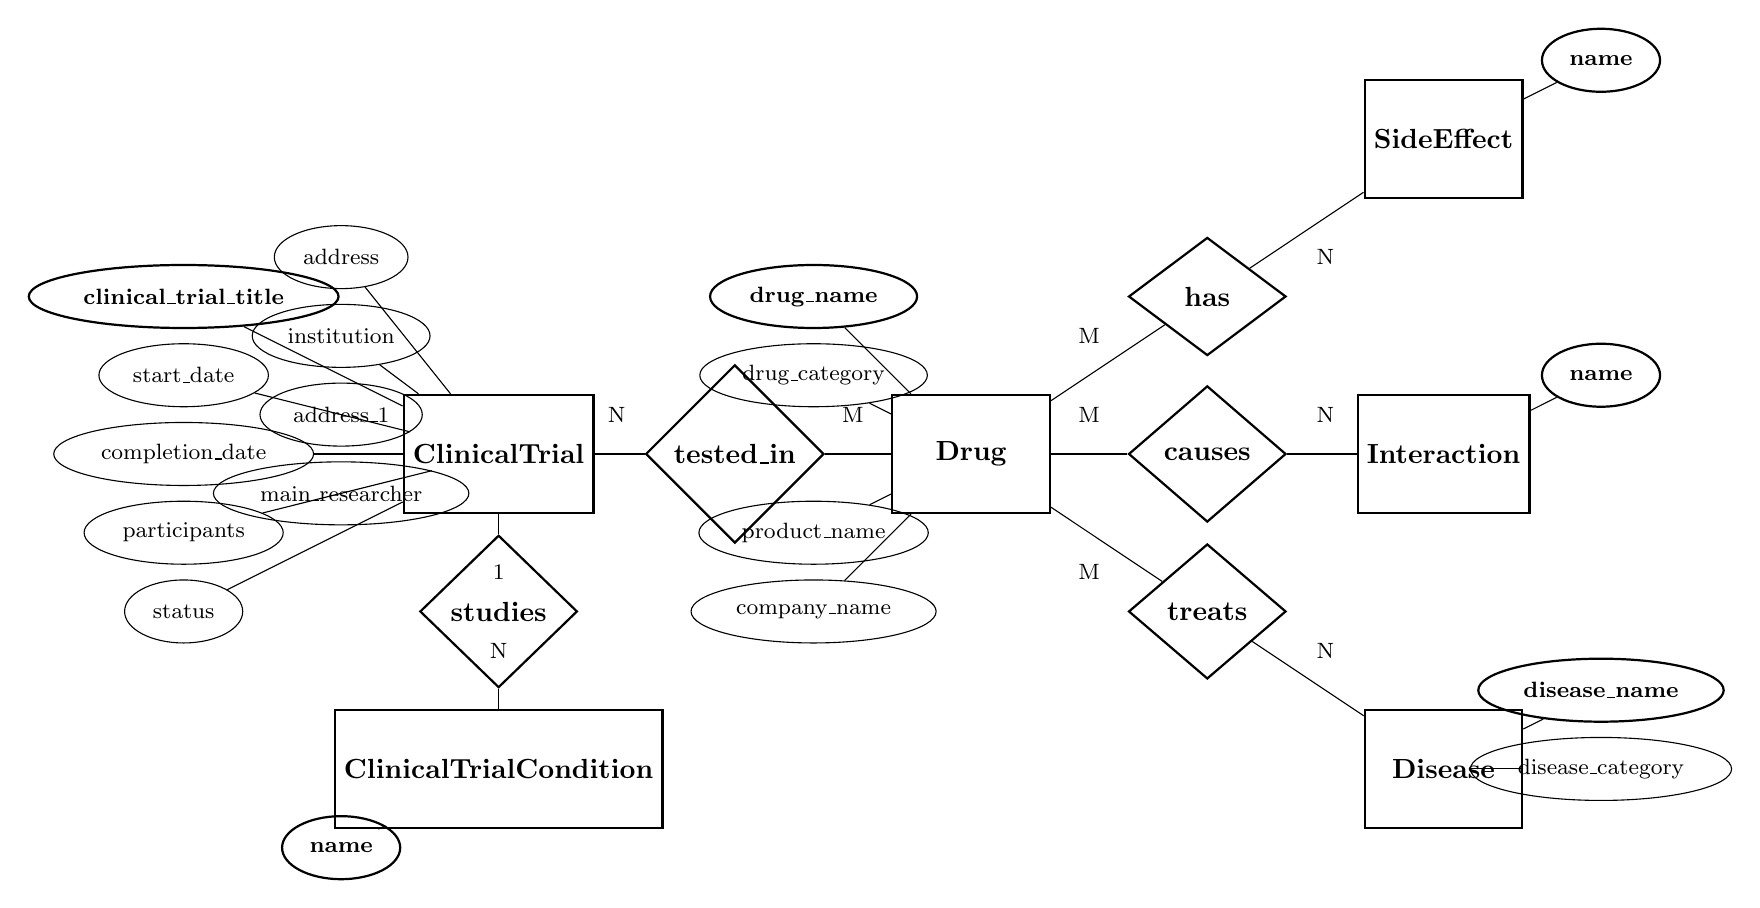
\begin{tikzpicture}[
    % Define styles
    entity/.style={rectangle, draw, thick, minimum width=2cm, minimum height=1.5cm, text centered, font=\bfseries},
    attribute/.style={ellipse, draw, minimum width=1.5cm, minimum height=0.8cm, text centered, font=\footnotesize},
    key_attribute/.style={ellipse, draw, thick, minimum width=1.5cm, minimum height=0.8cm, text centered, font=\footnotesize\bfseries},
    relationship/.style={diamond, draw, thick, minimum width=2cm, minimum height=1.5cm, text centered, font=\bfseries},
    line/.style={-},
    arrow/.style={-stealth}
]

% Main Entities
\node[entity] (drug) at (0,0) {Drug};
\node[entity] (sideeffect) at (6,4) {SideEffect};
\node[entity] (interaction) at (6,0) {Interaction};
\node[entity] (disease) at (6,-4) {Disease};
\node[entity] (clinicaltrial) at (-6,0) {ClinicalTrial};
\node[entity] (condition) at (-6,-4) {ClinicalTrialCondition};

% Drug Attributes
\node[key_attribute] (drug_name) at (-2,2) {drug\_name};
\node[attribute] (drug_category) at (-2,1) {drug\_category};
\node[attribute] (product_name) at (-2,-1) {product\_name};
\node[attribute] (company_name) at (-2,-2) {company\_name};

% SideEffect Attributes
\node[key_attribute] (se_name) at (8,5) {name};

% Interaction Attributes
\node[key_attribute] (int_name) at (8,1) {name};

% Disease Attributes
\node[key_attribute] (disease_name) at (8,-3) {disease\_name};
\node[attribute] (disease_category) at (8,-4) {disease\_category};

% ClinicalTrial Attributes
\node[key_attribute] (ct_title) at (-10,2) {clinical\_trial\_title};
\node[attribute] (ct_start) at (-10,1) {start\_date};
\node[attribute] (ct_completion) at (-10,0) {completion\_date};
\node[attribute] (ct_participants) at (-10,-1) {participants};
\node[attribute] (ct_status) at (-10,-2) {status};
\node[attribute] (ct_address) at (-8,2.5) {address};
\node[attribute] (ct_institution) at (-8,1.5) {institution};
\node[attribute] (ct_address1) at (-8,0.5) {address\_1};
\node[attribute] (ct_researcher) at (-8,-0.5) {main\_researcher};

% ClinicalTrialCondition Attributes
\node[key_attribute] (cond_name) at (-8,-5) {name};

% Relationships
\node[relationship] (has_side_effect) at (3,2) {has};
\node[relationship] (has_interaction) at (3,0) {causes};
\node[relationship] (treats) at (3,-2) {treats};
\node[relationship] (tested_in) at (-3,0) {tested\_in};
\node[relationship] (studies) at (-6,-2) {studies};

% Connect Drug to its attributes
\draw[line] (drug) -- (drug_name);
\draw[line] (drug) -- (drug_category);
\draw[line] (drug) -- (product_name);
\draw[line] (drug) -- (company_name);

% Connect SideEffect to its attributes
\draw[line] (sideeffect) -- (se_name);

% Connect Interaction to its attributes
\draw[line] (interaction) -- (int_name);

% Connect Disease to its attributes
\draw[line] (disease) -- (disease_name);
\draw[line] (disease) -- (disease_category);

% Connect ClinicalTrial to its attributes
\draw[line] (clinicaltrial) -- (ct_title);
\draw[line] (clinicaltrial) -- (ct_start);
\draw[line] (clinicaltrial) -- (ct_completion);
\draw[line] (clinicaltrial) -- (ct_participants);
\draw[line] (clinicaltrial) -- (ct_status);
\draw[line] (clinicaltrial) -- (ct_address);
\draw[line] (clinicaltrial) -- (ct_institution);
\draw[line] (clinicaltrial) -- (ct_address1);
\draw[line] (clinicaltrial) -- (ct_researcher);

% Connect ClinicalTrialCondition to its attributes
\draw[line] (condition) -- (cond_name);

% Connect entities through relationships
\draw[line] (drug) -- (has_side_effect);
\draw[line] (has_side_effect) -- (sideeffect);

\draw[line] (drug) -- (has_interaction);
\draw[line] (has_interaction) -- (interaction);

\draw[line] (drug) -- (treats);
\draw[line] (treats) -- (disease);

\draw[line] (drug) -- (tested_in);
\draw[line] (tested_in) -- (clinicaltrial);

\draw[line] (clinicaltrial) -- (studies);
\draw[line] (studies) -- (condition);

% Add cardinality labels
\node[font=\footnotesize] at (1.5,1.5) {M};
\node[font=\footnotesize] at (4.5,2.5) {N};

\node[font=\footnotesize] at (1.5,0.5) {M};
\node[font=\footnotesize] at (4.5,0.5) {N};

\node[font=\footnotesize] at (1.5,-1.5) {M};
\node[font=\footnotesize] at (4.5,-2.5) {N};

\node[font=\footnotesize] at (-1.5,0.5) {M};
\node[font=\footnotesize] at (-4.5,0.5) {N};

\node[font=\footnotesize] at (-6,-1.5) {1};
\node[font=\footnotesize] at (-6,-2.5) {N};

\end{tikzpicture}




\section*{6.24 Airline Database}
\begin{tikzpicture}[
    node distance=2.5cm,
    entity/.style={rectangle, draw, minimum width=2cm, minimum height=0.8cm, text centered},
    relationship/.style={diamond, draw, minimum width=2cm, minimum height=0.8cm, text centered},
    attribute/.style={ellipse, draw, minimum width=1.5cm, minimum height=0.6cm, text centered, font=\small},
    key/.style={ellipse, draw, minimum width=1.5cm, minimum height=0.6cm, text centered, font=\small, text decoration=underline}
]

% Entities
\node[entity] (customer) {Customer};
\node[entity, right=6cm of customer] (flights) {Flights};

% Relationships
\node[relationship, right=1.5cm of customer] (reservation) {Reservation};

% Customer attributes
\node[key, above left=1cm of customer] (customer_id) {\underline{customer\_id}};
\node[attribute, above=1cm of customer] (name) {name};
\node[multivalued attribute, below left=1.2cm of customer] (phone_number) {phone number};
\node[attribute, below=1cm of customer] (address) {address};

% Flights attributes
\node[key, above left=1cm of flights] (flight_id) {\underline{flight\_id}};
\node[attribute, above=1cm of flights] (source) {source};
\node[attribute, above right=1cm of flights] (destination) {destination};
\node[attribute, below =1.3cm of flights] (timestamp_src) {timestamp src};
\node[attribute, below right=1cm of flights] (timestamp_dest) {timestamp dest};

% Connections
\draw (customer) -- (reservation);
\draw (reservation) -- (flights);

% Attribute connections
\draw (customer) -- (customer_id);
\draw (customer) -- (name);
\draw (customer) -- (phone_number);
\draw (customer) -- (address);
\draw (flights) -- (flight_id);
\draw (flights) -- (source);
\draw (flights) -- (destination);
\draw (flights) -- (timestamp_src);
\draw (flights) -- (timestamp_dest);

\end{tikzpicture}

\newpage

% ============================================================================
% 6.26 Motor Vehicle Sales Company - Generalization-Specialization Hierarchy
% ============================================================================
\section*{6.26 Motor Vehicle Sales Company}
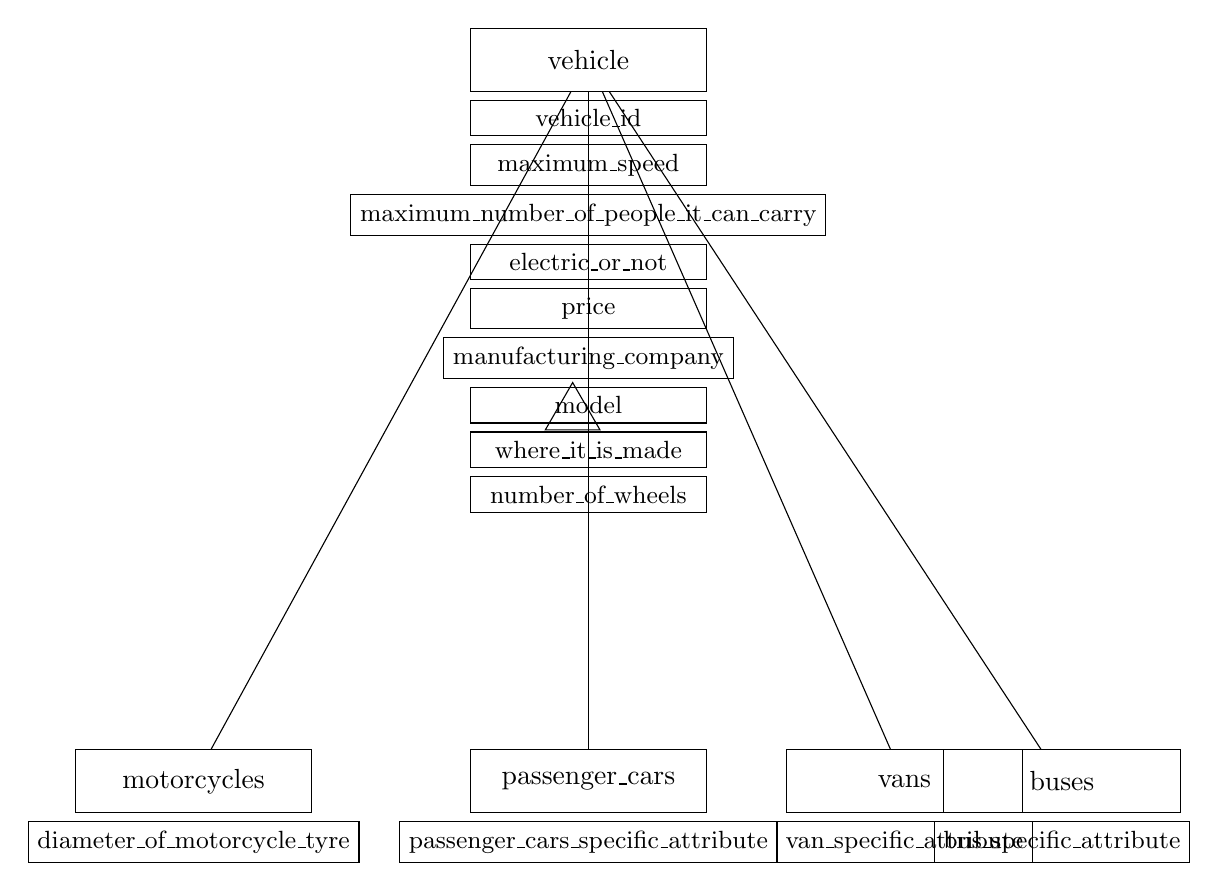
\begin{tikzpicture}[
    node distance=2cm,
    entity/.style={rectangle, draw, minimum width=3cm, minimum height=0.8cm, text centered},
    attribute/.style={rectangle, draw, minimum width=3cm, minimum height=0.4cm, text centered, font=\small}
]

% Main Vehicle entity
\node[entity] (vehicle) at (0,0) {vehicle};

% Vehicle attributes
\node[attribute, below=0.1cm of vehicle] (vehicle_id) {vehicle\_id};
\node[attribute, below=0.1cm of vehicle_id] (max_speed) {maximum\_speed};
\node[attribute, below=0.1cm of max_speed] (max_people) {maximum\_number\_of\_people\_it\_can\_carry};
\node[attribute, below=0.1cm of max_people] (electric) {electric\_or\_not};
\node[attribute, below=0.1cm of electric] (price) {price};
\node[attribute, below=0.1cm of price] (manufacturing) {manufacturing\_company};
\node[attribute, below=0.1cm of manufacturing] (model) {model};
\node[attribute, below=0.1cm of model] (where_made) {where\_it\_is\_made};
\node[attribute, below=0.1cm of where_made] (num_wheels) {number\_of\_wheels};

% Specialization entities
\node[entity, below left=3cm and 2cm of num_wheels] (motorcycles) {motorcycles};
\node[entity, below=3cm of num_wheels] (passenger_cars) {passenger\_cars};
\node[entity, below right=3cm and 1cm of num_wheels] (vans) {vans};
\node[entity, below right=3cm and 3cm of num_wheels] (buses) {buses};

% Specialization attributes
\node[attribute, below=0.1cm of motorcycles] (diameter) {diameter\_of\_motorcycle\_tyre};
\node[attribute, below=0.1cm of passenger_cars] (passenger_attr) {passenger\_cars\_specific\_attribute};
\node[attribute, below=0.1cm of vans] (van_attr) {van\_specific\_attribute};
\node[attribute, below=0.1cm of buses] (bus_attr) {bus\_specific\_attribute};

% ISA relationship lines
\draw (vehicle) -- (motorcycles);
\draw (vehicle) -- (passenger_cars);
\draw (vehicle) -- (vans);
\draw (vehicle) -- (buses);

% ISA triangle
\node[regular polygon, regular polygon sides=3, draw, minimum size=0.8cm] at (-0.2,-4.5) {};

\end{tikzpicture}

\end{document}
